\documentclass[conference]{IEEEtran}
\IEEEoverridecommandlockouts
% The preceding line is only needed to identify funding in the first footnote. If that is unneeded, please comment it out.
\usepackage{xcolor}
% \usepackage{ulem}
\definecolor{bleudefrance}{rgb}{0.19, 0.55, 0.91}
\newcommand\vitor[1]{{\textcolor{red}{[{#1}]}}}
\newcommand\matheus[1]{{\textcolor{bleudefrance}{[{#1}]}}}

\usepackage{cite}
\usepackage{amsmath,amssymb,amsfonts}
\usepackage{algorithmic}
\usepackage{graphicx}
\usepackage{textcomp}
\usepackage{booktabs}
\usepackage{xcolor}
\usepackage{url}
\def\BibTeX{{\rm B\kern-.05em{\sc i\kern-.025em b}\kern-.08em
    T\kern-.1667em\lower.7ex\hbox{E}\kern-.125emX}}
\begin{document}



\title{Classificando terrenos por meio de imagens aéreas}


\author{\IEEEauthorblockN{Matheus Peixoto Ribeiro Vieira}
\IEEEauthorblockA{\textit{Departamento de Computação (DECOM)} \\
\textit{Universidade Federal de Ouro Preto}\\
Ouro Preto, Brasil \\
matheus.peixoto@aluno.ufop.edu.br}
\and
\IEEEauthorblockN{Vitor Oliveira Diniz}
\IEEEauthorblockA{\textit{Departamento de Computação (DECOM)} \\
\textit{Universidade Federal de Ouro Preto}\\
Ouro Preto, Brasil \\
vitor.diniz@aluno.ufop.edu.br}

}

\maketitle

\begin{abstract}
O uso de imagens aéreas tem se mostrado essencial para o enfrentamento de desafios ambientais, humanitários e de segurança em regiões extensas como a Amazônia. Este trabalho propõe um modelo de classificação automática de cenas aéreas utilizando técnicas de aprendizado de máquina aplicadas ao Aerial Image Dataset (AID), com o objetivo de categorizar diferentes tipos de cobertura do solo de forma precisa e eficiente. A abordagem visa superar limitações de inspeções tradicionais, oferecendo suporte a decisões estratégicas em situações como desmatamento ilegal, desastres climáticos e conflitos geopolíticos. O estudo envolve uma revisão de métodos recentes, seleção e pré-processamento do AID, treinamento e avaliação de modelos com métricas padronizadas, e comparação com trabalhos relacionados. Os resultados apontam o potencial da classificação automatizada para transformar imagens de satélite em informações acionáveis, otimizando ações de monitoramento e resposta em tempo real.
\end{abstract}

\begin{IEEEkeywords}
Imagens aéreas, AID, classificação
\end{IEEEkeywords}

\section{Introdução}
    O uso de imagens de satélite tem se tornado cada vez mais crucial para o planejamento de políticas públicas, especialmente em regiões de grandes dimensões como a Amazônia. O desmatamento anual da floresta amazônica atingiu níveis sem precedentes, ultrapassando 10 000 \(km^{2}\) por ano entre 2019 e 2021, um aumento de 56,6\% em relação ao triênio anterior \cite{ipam2022}. Somente em terras públicas não destinadas foram perdidos, em média, 3 933 km² de floresta por ano, evidenciando a necessidade de monitoramento automatizado e em tempo real para apoiar ações de fiscalização e comando e controle.

    Além do monitoramento ambiental, o emprego de imagens aéreas é fundamental para revelar infraestruturas clandestinas que sustentam atividades ilegais. Na Terra Indígena Yanomami, por exemplo, pistas de pouso improvisadas vêm sendo utilizadas para o transporte de equipamentos e suprimentos a garimpos ilegais, gerando violência contra as populações locais e degradação ambiental massiva \cite{bastos2024}.

    Nos últimos anos, o clima extremo também vem causando impactos drásticos na sociedade. Em abril e maio de 2024, 90\% do território do Rio Grande do Sul foi inundado, deslocando mais de 581 000 pessoas e causando 169 mortes confirmadas em um evento atribuído à conjugação de El Niño, bloqueios atmosféricos e aquecimento global \cite{fearnside2024}. Com informações capturadas por satélite em tempo real, seria possível mapear as áreas de risco, priorizar evacuações e otimizar o envio de recursos de emergência.

    Mais recentemente, conflitos geopolíticos – como o escalonamento de ataques entre Israel e Irã, com mortes de líderes militares e atingimento de instalações nucleares, seguidos de retaliações mútuas – reforçam a importância de uma visão integrada do território a partir de imagens aéreas. Governos soberanos dependem desse tipo de inteligência geoespacial não apenas para defender fronteiras, mas também para planejar infraestrutura crítica e proteger a população \cite{g1_2025_israel_x_ira,g1_2025_israel_ataque_ira,bbc2025_eua_ataque_tehera,bbc2025_ira_retalia}.

    A extensão continental da Amazônia e de outras regiões críticas impõe barreiras logísticas e operacionais que tornam ineficazes as respostas reativas tradicionais. Inspeções de campo e sobrevoos rotineiros demandam tempo e recursos que não acompanham o ritmo acelerado dos eventos de desmatamento, inundação ou ocupação ilegal. A classificação automatizada sobre imagens de alta resolução é, portanto, essencial para identificar rapidamente hotspots de atividade anômala e orientar equipes móveis de fiscalização e socorro.
    
    Em síntese, a classificação automática de cenas aéreas representa uma ferramenta poderosa não apenas para transformar grandes volumes de dados de satélite em \textit{insights} acionáveis, mas também para permitir uma atuação preventiva e direcionada diante de desafios ambientais, humanitários e de segurança. Ao categorizar com precisão diferentes usos e coberturas do solo, este trabalho demonstra como técnicas de Machine Learning aplicadas ao AID podem embasar decisões estratégicas e antecipar-se a crises antes que se tornem catástrofes.


    
\section{Objetivo}
    Este trabalho tem por objetivo o desenvolvimento de um modelo capaz de classificar diferentes imagens aéreas de acordo com o local que se referem. Para isso, os seguintes objetivos específicos são propostos

    \begin{itemize}
        \item Explorar a literatura para identificar técnicas de classificação e \textit{datasets} disponíveis;
        \item Determinar um conjunto de dados para ser explorado;
        \item Propor, treinar e avaliar um modelo meio de métricas de acurácia global e outras métricas padronizadas de classificação;
        \item Comparar os resultados obtidos com os trabalhos relacionados;
        \item Identificar pontos fortes e limitações do método proposto, propondo diretrizes para futuras melhorias e ampliações do conjunto de dados e da arquitetura de classificação.
    \end{itemize}

\section{Trabalhos relacionados}\label{trabalhos_relacionados}

    Propondo uma abordagem leve e eficiente para a classificação de imagens aéreas, \cite{b4} aproveita camadas específicas de um modelo pré-treinado da MobileNetV2, que, com base na razão de zeros antes e depois da ativação ReLU no \textit{batch normalization} de algumas camadas, as que possuem o maior valor indicam que os dados podem ser mais representativos, logo elas são salvas. Dessa forma, as imagens são passadas por essas camadas e seus resultados passam por um \textit{global average pooling} e uma redução de tamanho por PCA e LDA, diminindo o tamanho do vetor de características, que alimenta uma SVM para predizer a classe da imagem em uma configuração one-vs-rest. Assim, foi possível obter uma acurácia de 93,64\% no \textit{dataset} AID e 88,05\% no NWPU. 

    Em diferentes conjuntos de dados de imagens áreas, é comum a presença de ambiguidade nos dados. Ou seja, uma figura de uma área residencial pode possuir estradas, o que pode ser confundível com uma zona comercial. Levando em consideração tal desafio, \cite{b3}, não utiliza rótulos únicos para cada imagem, mas sim uma distribuição baseada na similaridade visual e na correlação entre rótulos de vizinhos próximos, que são combinadas com o rótulo original. Depois os dados são treinados em redes convolucionais e usa uma função de erro que mistura \textit{cross-entropy} e  divergência KL. Com isso, foi possível obter uma acurácia de 94,11\% no dataset AID, 89,80\% no NWPU
    
    Para gerar uma maior quantidade de imagens para treino, \cite{b2} propôs diferentes formas de \textit{data augmentation} com CutOut (Remoção de uma parte aleatória da imaagem), MixUp (Sobreposição de uma imagem com outra por interpolação) e CutMix (Recrota parte de uma imagem e cola em outra). Com o uso de \textit{Vision Transformers} para a extração de características, foi possível obter uma acurácia de até 98,48\% no \textit{dataset} Merced, 95,86\% no AID e 95,56\% no Optimal31. Também foi mostrado que a redução no número de camadas do \textit{transformer} ainda pode mantê-lo com resultados competitivos.

    Em um conjunto de dados de visão área de uma igreja, a mesma pode estar mais próxima ou mais distante, variando muito de acordo com a maneira que a imagem foi capturada. Portanto, \cite{b1} propõe um modelo que utiliza um ViT para lidar com as escalas locais dos itens, usando um \textit{patch-size} \textit{small} e outro \textit{large}, e um modelo totalmente conectado que recebe uma versão menor da imagem para realizar uma análise global da mesma. Os dados são agrupados por um mecanismo de \textit{self-attention} e uma função de \textit{loss} garante a a consistência entre ambas saídas. Assim, com tal modelo foi possível obter uma acurácia de 99,93\% no UCM, 97,67\% no AID e 95,60\% no NWPU.

    Uma abordagem conjunta de extração local e global de informações utilizando dois ramos distintos de um mesmo modelo é explorado em \cite{b0}. Faz a extração de informações por um  Vision Transformer (ViT), enquanto faz uma extração local por uma rede convolucional pré-treinada, como a ResNet34 ou a MobileNetV2. As características extraídas por ambos os ramos são então concatenadas para compor uma representação conjunta, que é utilizada na predição final. Durante o treinamento, cada ramo também realiza predições individualmente, sendo otimizadas com funções de perda baseadas em entropia cruzada. Para garantir a compatibilidade e coesão entre os dois espaços de representação, é empregada adicionalmente a Center loss em ambos os ramos, promovendo uma maior agregação intra-classe. Essa estratégia conjunta permitiu ao modelo alcançar uma acurácia de 95,49\% no conjunto NWPU e de 97,70\% no conjunto AID.

    \begin{table}[!htb]
        \centering
        \begin{tabular}{@{}ccccc@{}}
            \toprule
            \textbf{Artigo} & \textbf{Metodologia} & \textbf{Base de dados} & \textbf{Acurácia} \\ \midrule
            \cite{b4} & CNN + PCA + LDA + SVM & AID \cite{aidDataset} & 93,64\% \\
                      &                        & NWPU \cite{nwpuDataset} & 88,05\% \\ \midrule
                                              
            \cite{b3} & Redes Convolucionais & AID \cite{aidDataset} & 94,11\% \\
                     &                       & NWPU \cite{nwpuDataset} & 89,90\% \\ \midrule
                     
            \cite{b2} & Vision Transformers & Merced \cite{mercedDataset} & 98,48\% \\
                     &                      & AID \cite{aidDataset} & 95,86\% \\
                     &                      & Optimal31 \cite{optimal31Dataset} & 95,56\% \\  \midrule
                     
            \cite{b1} & Vision Transformers + Redes Neurais & UCM \cite{ucmDataset} & 99,93\% \\
                     &                                      & AID \cite{aidDataset} & 97,67\% \\
                     &                                      & NWPU \cite{nwpuDataset} & 95,60\% \\  \midrule
                     
            \cite{b0} & Vision Transformers + CNNs & NWPU \cite{nwpuDataset} & 95,49\% \\
                     &                             & AID \cite{aidDataset} & 97,70\% \\ \bottomrule
        \end{tabular}
        \caption{Resumo de metodologias e acurácias em diferentes bases de dados.}
        \label{tab:resultados_artigos}
    \end{table}

    A tabela \ref{tab:resultados_artigos} exibe uma sumarização das metodologias aplicadas em cada um dos trabalhos mencionados acima juntamente com seus resultados obtidos. Assim, observa-se acurácias altas, indicando uma boa generalização dos modelos propostos. Todavia, essa métrica analisada unicamente pode ser enviesada e uma classe pode ter sido errada completamente, mas devido à grande presença de classes, esses valores podem ser mascarados.

\section{Conjunto de dados}

    O \textit{Aerial Image Dataset} (AID) é um conjunto de dados de imagens aéreas para a classificação de áreas. Ele possui 10.000 imagens RGB com resolução de \(600 \times 600\), sendo que a resolução varia entre 0,5 e 8 metros por pixel, ou seja, em algumas imagens, um pixel corresponde a 0,5 metros, e, em outras, corresponde a 8 metros. Entre as suas 30 diferentes classes, a quantidade de imagens varia de 220 a 420, com uma média de 333 imagens por classe e um desvio padrão de 56.8 imagens. 
    
    Os dados foram coletados de imagens do Google Earth e possui 30 diferentes classes, como aeroportos, florestas, estacionamentos, igrejas, campos de futebol, etc. As imagens são de países diversos como Alemanha, China, Estados Unidos, França e Japão, com diferentes estações do ano, iluminação, escala e orientação.

    Por fim, o \textit{dataset} propõe um desafio maior ao possuir uma alta variação entre os elementos de uma mesma classe, ao passo em que possui elementos semelhantes em imagens de diferentes classes, aumentando a complexidade do mesmo, como ocorre com as figuras \ref{fig:playground} e \ref{fig:estadio}, que pertencem a classes diferentes (\textit{Playground} e Estádio, respectivamente), mas possuem características semelhantes, como o campo de futebol no centro e uma pista de atletismo ao lado.

    \begin{figure}[!htb]
        \centering
        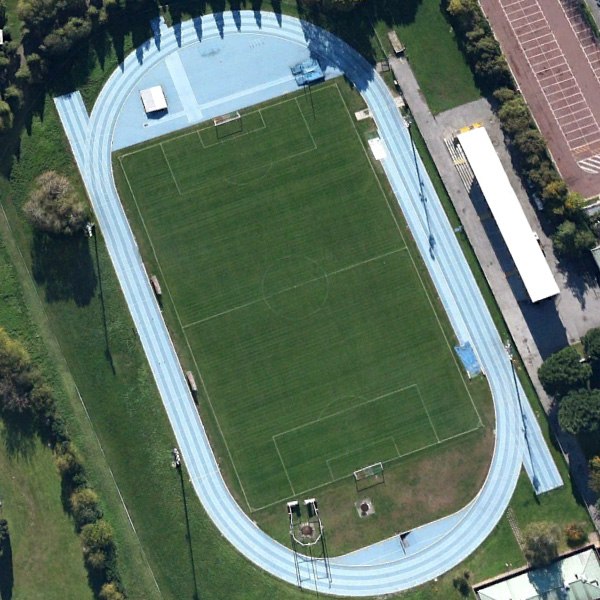
\includegraphics[width=0.5\linewidth]{Images/playground_184.jpg}
        \caption{\textit{Playground}}
        \label{fig:playground}
    \end{figure}

    \begin{figure}[!htb]
        \centering
        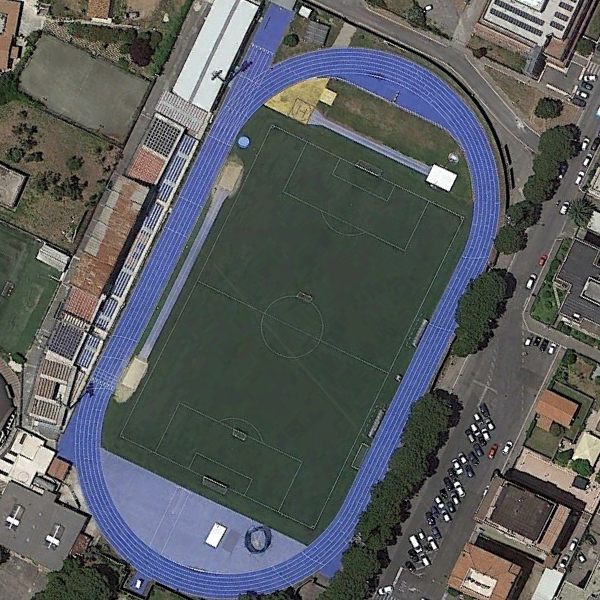
\includegraphics[width=0.5\linewidth]{Images/stadium_247.jpg}
        \caption{Estádio}
        \label{fig:estadio}
    \end{figure}





\section{Referencias}
\begin{thebibliography}{00}

    \bibitem{aidDataset} G.-S. Xia, J. Hu, F. Hu, B. Shi, X. Bai, Y. Zhong, L. Zhang, and X. Lu, ``AID: A benchmark data set for performance evaluation of aerial scene classification,'' *IEEE Trans. Geosci. Remote Sens.*, vol. 55, no. 7, pp. 3965--3981, Jul. 2017.

    \bibitem{nwpuDataset} G. Cheng, J. Han and X. Lu, "Remote Sensing Image Scene Classification: Benchmark and State of the Art," in Proceedings of the IEEE, vol. 105, no. 10, pp. 1865-1883, Oct. 2017, doi: 10.1109/JPROC.2017.2675998.

    \bibitem{ucmDataset} Y. Yang and S. Newsam, “Geographic image retrieval using local invariant features,” IEEE Trans. Geosci. Remote Sens., vol. 51, no. 2, pp. 818–832, Feb. 2013.

    \bibitem{optimal31Dataset} Braj Raj Nagar, "optimal-31", avilable in: www.kaggle.com/datasets/brajrajnagar/optimal-31, access on 24-06-2025

    \bibitem{mercedDataset} Yang, Y.; Newsam, S. Bag-of-visual-words and spatial extensions for land-use classification. In Proceedings of the 18th SIGSPATIAL International Conference on Advances in Geographic Information Systems—GIS ’10, San Jose, CA, USA, 2–5 November 2010; p. 270.


    \bibitem{b0}P. Deng, K. Xu and H. Huang, "When CNNs Meet Vision Transformer: A Joint Framework for Remote Sensing Scene Classification," in IEEE Geoscience and Remote Sensing Letters, vol. 19, pp. 1-5, 2022, Art no. 8020305, doi: 10.1109/LGRS.2021.3109061.

    \bibitem{b1}T. Peng, J. Yi and Y. Fang, "A Local–Global Interactive Vision Transformer for Aerial Scene Classification," in IEEE Geoscience and Remote Sensing Letters, vol. 20, pp. 1-5, 2023, Art no. 6004405, doi: 10.1109/LGRS.2023.3266008.
    
    \bibitem{b2}Bazi Y, Bashmal L, Rahhal MMA, Dayil RA, Ajlan NA. Vision Transformers for Remote Sensing Image Classification. Remote Sensing. 2021; 13(3):516. https://doi.org/10.3390/rs13030516 
    
    \bibitem{b3}Luo J, Wang Y, Ou Y, He B, Li B. Neighbor-Based Label Distribution Learning to Model Label Ambiguity for Aerial Scene Classification. Remote Sensing. 2021; 13(4):755. https://doi.org/10.3390/rs13040755 

    \bibitem{b4} M. A. Arefeen, S. T. Nimi, M. Y. S. Uddin and Z. Li, "A Lightweight Relu-Based Feature Fusion For Aerial Scene Classification," 2021 IEEE International Conference on Image Processing (ICIP), Anchorage, AK, USA, 2021, pp. 3857-3861, doi: 10.1109/ICIP42928.2021.9506524.

    \bibitem{ipam2022}  
    A. Alencar, R. Silvestrini, J. Gomes and G. Savian,  
    “Amazônia em Chamas: O Novo e Alarmante Patamar do Desmatamento na Amazônia,”  
    Instituto de Pesquisa Ambiental da Amazônia (IPAM), Nota Técnica nº 9, fev. 2022.

  \bibitem{bastos2024}  
    E. Bastos Furtado, T. Franchi, L. Barreto Rodrigues and G. Da Frota Simões,  
    “Asas que Devastam a Amazônia: Uma Análise do Cenário de Pistas de Pouso e Voos Irregulares que Dão Suporte ao Garimpo Ilegal na TI Yanomami,”  
    Revista (RE)DEFINIÇÕES DAS FRONTEIRAS, vol. 2, no. 6, pp. 16–43, jan. 2024.

  \bibitem{fearnside2024}  
    P. M. Fearnside and R. A. Silva,  
    “Surpresas Climáticas: a Amazônia e as Lições da Enchente Catastrófica no Rio Grande do Sul,”  
    3 jul. 2024. [Online]. Available: \url{https://amazoniareal.com.br/licoes-da-enchente-catastrofica-no-rio-grande-do-sul/}

  \bibitem{g1_2025_israel_x_ira}  
    G1,  
    “Israel x Irã: tudo o que se sabe até o momento sobre o conflito,”  
    G1, 18 jun. 2025. [Online]. Available: \url{https://g1.globo.com/mundo/noticia/2025/06/18/israel-x-ira-tudo-o-que-se-sabe-ate-o-momento-sobre-o-conflito.ghtml}

  \bibitem{g1_2025_israel_ataque_ira}  
    G1,  
    “Israel realiza ataque aéreo contra Irã,”  
    G1, 12 jun. 2025. [Online]. Available: \url{https://g1.globo.com/mundo/noticia/2025/06/12/israel-realiza-aereo-contra-ira.ghtml}

  \bibitem{bbc2025_eua_ataque_tehera}  
    BBC News Brasil,  
    “EUA atacam instalações nucleares de Teerã,”  
    jun. 2025. [Online]. Available: \url{https://www.bbc.com/portuguese/articles/c3r9qgjwevdo}

  \bibitem{bbc2025_ira_retalia}  
    BBC News Brasil,  
    “Irã ataca bases militares dos EUA em retaliação,”  
    jun. 2025. [Online]. Available: \url{https://www.bbc.com/portuguese/articles/c0q8wwdldgpo}
    

\end{thebibliography}



% @article{Xia_2017,
%    title={AID: A Benchmark Data Set for Performance Evaluation of Aerial Scene Classification},
%    volume={55},
%    ISSN={1558-0644},
%    url={http://dx.doi.org/10.1109/TGRS.2017.2685945},
%    DOI={10.1109/tgrs.2017.2685945},
%    number={7},
%    journal={IEEE Transactions on Geoscience and Remote Sensing},
%    publisher={Institute of Electrical and Electronics Engineers (IEEE)},
%    author={Xia, Gui-Song and Hu, Jingwen and Hu, Fan and Shi, Baoguang and Bai, Xiang and Zhong, Yanfei and Zhang, Liangpei and Lu, Xiaoqiang},
%    year={2017},
%    month=jul, pages={3965–3981} 
% }


\end{document}
